In this chapter we want to give an impression how sensitive the model reacts to changes in the environment of the model. The robustness is demonstrated along three dimensions: First, we investigate the effect of a variation in a single model parameter; then we turn to the question whether there are differences in simulation results if the agents act synchronously or asynchronously; and finally we show the impact of scaling  the population size. 

For the robustness checks we compare the averaged time series of 10 batch runs over 5000 iterations for two key macroeconomic variables, output per capita and the unemployment rate. The general model set up is the same as has been used in Deliverable 9.1 for the innovation policy experiments (for a further discussion we refer to Deliverable 9.1 and the references listed there).  

\section{Parameter sensitivity}

In the academic debate on agent-based modeling the parameterization of agent based models is still vulnerable to criticism due to the high number of degrees of freedom. One way to deal with such criticism is to directly estimate and calibrate the model using empirically based parameter values wherever possible. This has been done in EURACE to a high extent, nonetheless there remain some parameters which have no empirical counterparts or that are chosen in order to stabilize the simulation or yield plausible outcomes. 

Which effect the variation of such a parameter potentially has on the simulation outcome is exemplified by varying a parameter used in the firm's production planning decision. Each Consumption goods producer determines once a month the delivery quantities for each mall. This decision is based on past demand quantities at all malls served by a firm and is formulated as a standard production and inventory planning model with stochastic demand that can be found in the standard management literature (see for example \cite{Nahmias_2008}). Every period the mall stock of a firm is replenished up to a level such that the probability of stock-out is at a specific level. This level, respectively the underlying quantile of the normal distribution is a model parameter in the EURACE model. This parameter induces production quantities, and therefore hiring and firing, and investments of firms. Hence it is a crucial driver of the qualitative features of the dynamics of the model.

In our standard set up this parameter is set to 0.842 corresponding to a stock-out probability of 20\%. In addition to the standard value and in order to investigate the sensitivity, we ran simulations with a probability of 90\%, 50\%, and 2.5\%. The stabilizing effect of a low stock-out probability can be seen in Figure~\ref{parameter_variation}. If the planned mall stock is only sufficient to satisfy the expected demand with a probability of 10\% (i.e. a stock-out probability of 90\%) the economy collapses, immediately leading to full unemployment. But a stock-out probability of 50\% already yields a completely different picture: The economy does not collapse, but output and unemployment oscillate with a constant cycle duration. With that probability the unemployment rate is already on a economically reasonable level. If the probability is decreased to a level of 20\% the oscillation of both variables disappears and leads to a further decrease of the unemployment rate and output increase, respectively. Yet another reduction from 20\% to 2.5\% does not change the result significantly. 

We carried out these robustness checks for several parameters to find plausible regions for them. A general point is that especially for those parameters driving the individual behavioral rules a elaborated robustness check is important as they influence the aggregated outcome of the simulation.

Summarizing, in this experiment we showed that the EURACE model is relatively robust against a change in the parametrization. We demonstrated the sensitivity to changes in model parameters by varying a parameter that is a crucial factor of the production planning of firms. As long as the parameter is set in an economically reasonable range, a variation does not change the performance, but outside of this range the outcome changes dramatically where in a very extreme case the simulation breaks down. 

\begin{figure}[t]
\begin{minipage}[b]{.46\linewidth}
\centering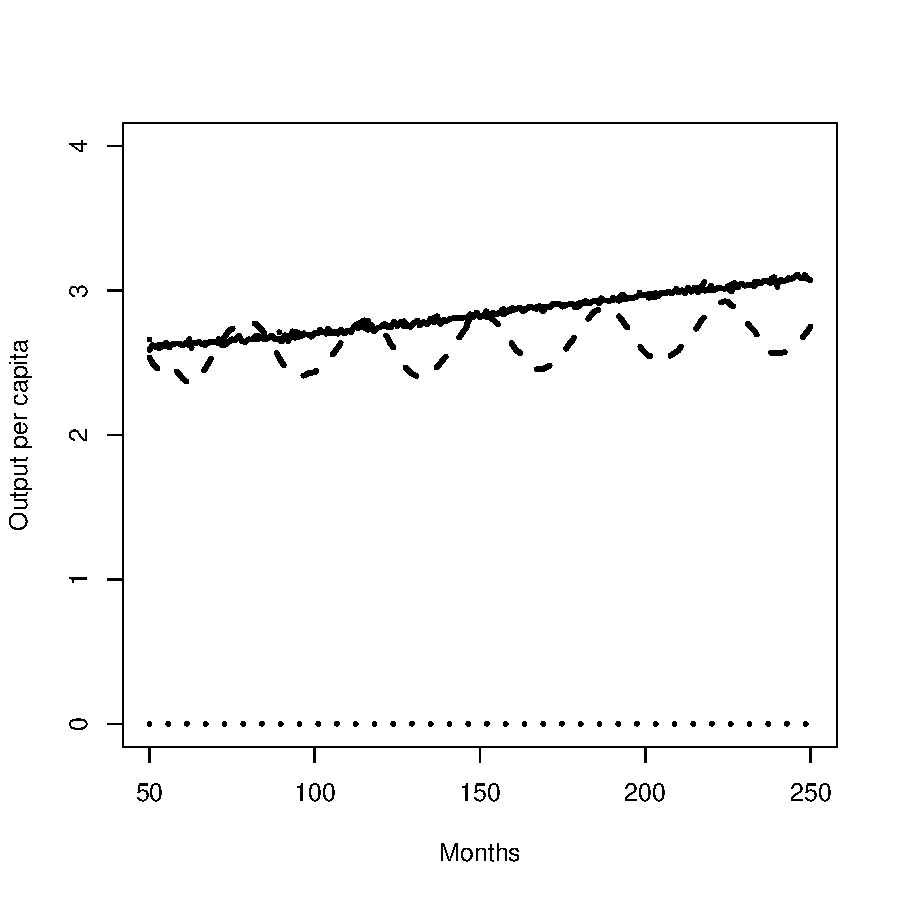
\includegraphics[scale =0.4]{./robustness/gdp_quantil.pdf}
\end{minipage}\hfill
\begin{minipage}[b]{.46\linewidth}
\centering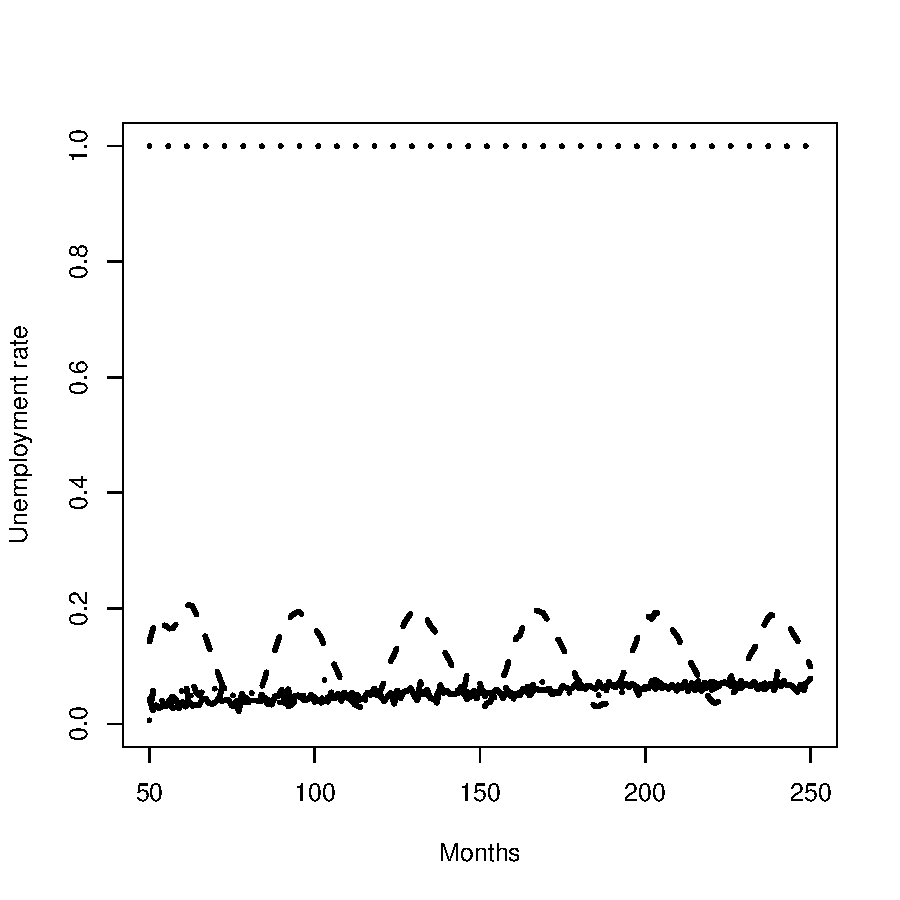
\includegraphics[scale=0.4]{./robustness/unemployment_quantil.pdf}
\end{minipage}
\caption{Sensitivity of the model to a variation in the stock-out probability on output per capita (left panel) and unemployment rate (right panel); 90 \% dotted line, 50\% dashed line, 20\% solid line, and 2.5\% dashed-dotted line.}
\label{parameter_variation}
\end{figure}

\section{Time synchronization}

In the second experiment we test if the time scale on which the agents make their decisions plays any role for the simulation outcome. In the majority of agent-based models there is a strong time-synchronization of actions because all agents make the same type of decisions simultaneously. In EURACE we have two different kinds of triggers for agent's actions: Event driven decisions are made if certain conditions in the agent's environment have changed and is reflected by a change in agent's memory (e.g. if a household becomes unemployed); however, most of the agent's decisions are calendar-time driven. This means there are fixed days in the month (respectively week or year) on which agents take certain actions. For example firms' decision about their monthly production quantities are made on fixed days of the month. These days of the month to act can vary between agents such that we have asynchronized production cycles. In the other case these days coincide such that we have synchronized activation days. The timing of production cycles has a high potential to influence the comparative performance since it sets the day when firms enter the labour, credit, financial and consumption goods market; consequently, this determines whether on all these markets the activities of agents are completely synchronized or not. The EURACE framework allows to explicitly study the aggregate effects of time-synchronization of individual behavior by varying these activation days.  

Figure~\ref{synchron_variation} shows the influence of an asynchronized versus synchronized decision making process of agents on the macroeconomic variables output per capita and unemployment rate. The effect is not that noticeable but especially the impact on the unemployment rate is verifiable. The unemployment is lower when decisions are made asynchroneously.

\begin{figure}[t]
\begin{minipage}[b]{.46\linewidth}
\centering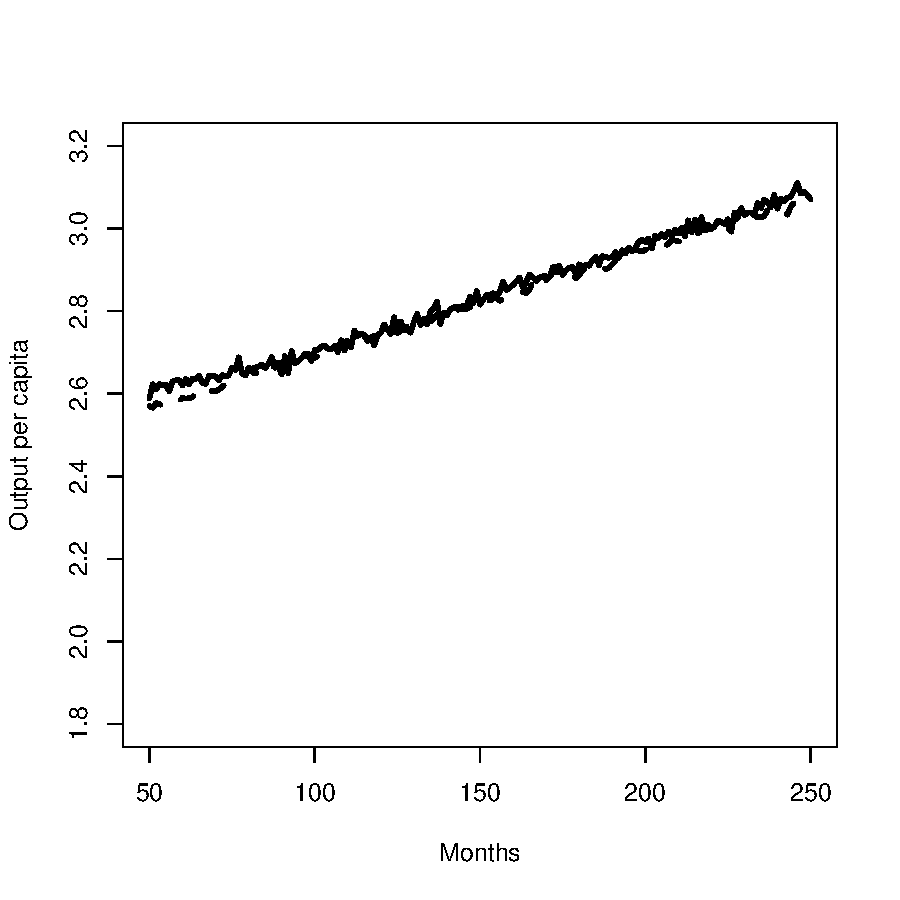
\includegraphics[scale =0.4]{./robustness/gdp_synchron.pdf}
\end{minipage}\hfill
\begin{minipage}[b]{.46\linewidth}
\centering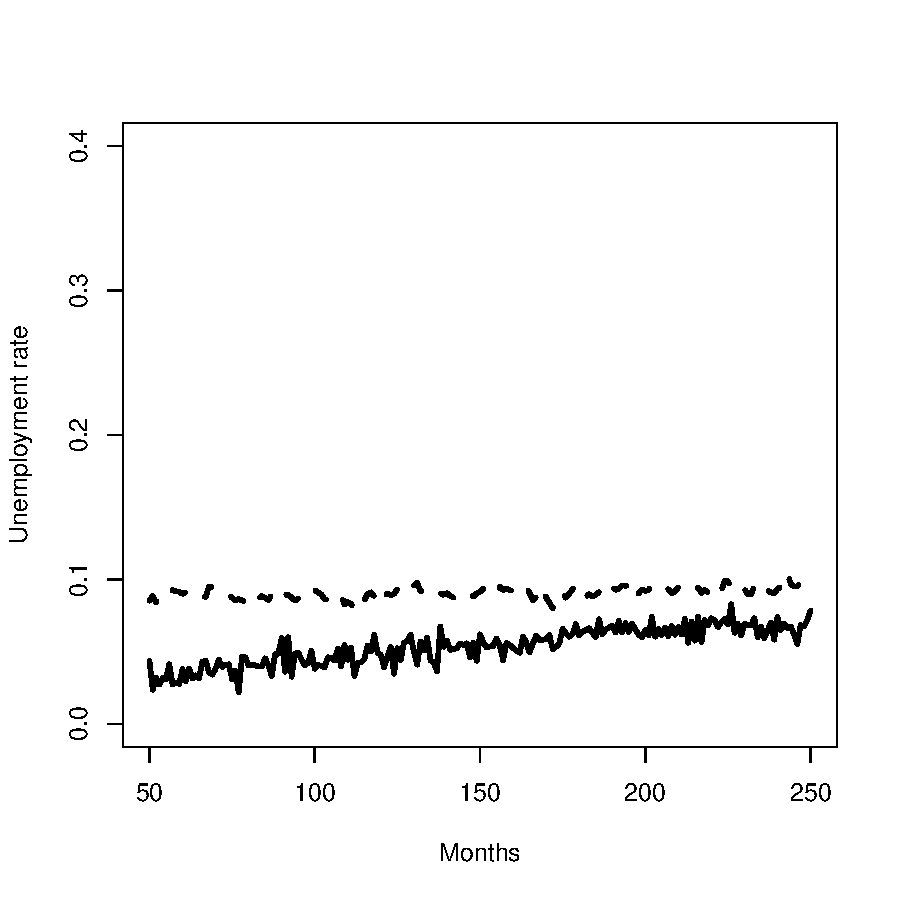
\includegraphics[scale=0.4]{./robustness/unemployment_synchron.pdf}
\end{minipage}
\caption{Differences in output per capita (left panel) and unemployment (right panel) of a asynchronized (solid line) versus synchronized (dashed line) decision making.}
\label{synchron_variation}
\end{figure}

\section{Population scaling}

The third experiment investigates the effect of scaling the population size thereby leaving the ratio between households and firms constant. Furthermore the initial production plan and the firm's endowment with capital and households' with wealth is not changed. 

A priori the impact of the population size is not clear but it should be a very important point of interest when talking about agent-based macroeconomic models. The computational effort to run and analyze large-scale agent-based models is still enormous, and from that perspective the question is still worthwhile if there are additional gains from large-scale simulations in fact. So the question that could be posed is: Is it necessary to run a macro model with an empirically reasonable number of agents or is a small scale model also able to generate the same insights? Note that \cite{Axtell_2000} makes the point that in order to reproduce the firm size distribution one needs at least several millions of workers, since empirically the largest firm (Wall Mart) has 1.5 million employees, and there are one million companies with one worker (self employed).     

Figure~\ref{scaling_variation} indicates that the EURACE model is very robust against a variation of the population size. In terms of output per capita there is just a small difference that establishes after month 150 (iteration 3000), where a scaling effect on the unemployment rate is not detectable. Thus, this final experiment pointed to the robustness against an increase in the number of agents in absolute terms where their relative number as well as the initial conditions are kept unchanged. 

This experiment suggests that the additional advantage seems to be small and a reasonable analysis of an agent-based macro model can be based on small scale models. In any case, this experiment was run with a maximum number of 10.000 households, far away from the empirical number of households in a real economy. 

A low sensitivity to a population scaling is true for the given model set up. The model used for these tests has only one region and all agents have the identical initial conditions. If the model is more refined in the sense that it is set up with more than one region and the initial memory of agents is set according to empirical distributions the population size might matter.  

\begin{figure}[t]
\begin{minipage}[b]{.46\linewidth}
\centering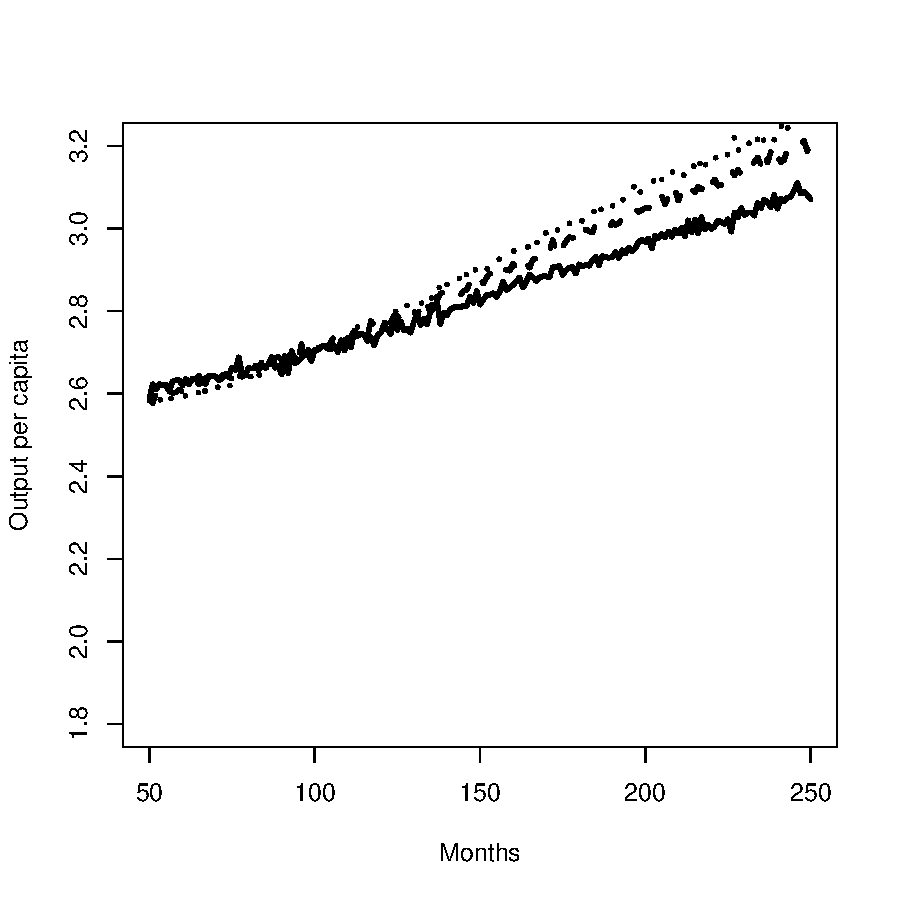
\includegraphics[scale =0.4]{./robustness/gdp_scaling.pdf}
\end{minipage}\hfill
\begin{minipage}[b]{.46\linewidth}
\centering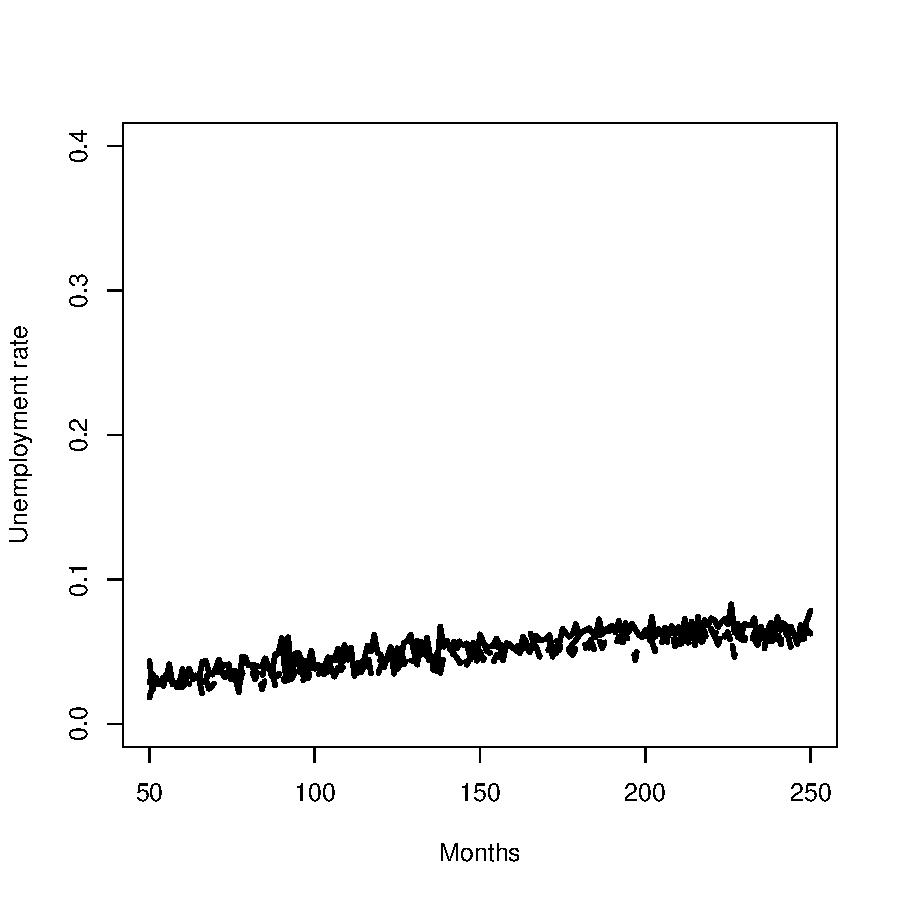
\includegraphics[scale=0.4]{./robustness/unemployment_scaling.pdf}
\end{minipage}
\caption{Impact of scaling of the agent population on aggregate output and unemployment; solid line 1600 households and 80 firms, dashed line 5000/250, and dotted line 10.000/500.}
\label{scaling_variation}
\end{figure}
